\documentclass{article}

\usepackage[utf8]{inputenc}

\usepackage[a4paper, total={6in, 10in}]{geometry}
\usepackage{amsmath}
\usepackage{hyperref}
\usepackage{graphicx}
\usepackage{tikz}
\usepackage{forest}

\usepackage{subcaption}

\title{Assignment 4}
\author{Abhi Patel, Andy Chen, Leroy Souz}

\date{12th Dec 2024}

\begin{document}

\maketitle

\section{Question 1}

\subsection

BOX LINKS:
Problem 1: \href{https://rutgers.box.com/s/65w22m50a3l7tqwhas2hipgy2nxr4mqa}{Problem 1 Link}
Problem 2: \href{https://rutgers.box.com/s/y57wu0mnwv7bddl0ayq6ks4p2ugvwd9i}{Problem 2 Link}

For generating a bitmap image for each number, we downloaded all the imaged from Digits and first resize the images to 7x12. Then, we decided to take the mean of all of the images per each digit. The reason we decided to do this was because we believed that calculating the mean image(using NumPy to calculate mean) would be the best representative of the defining features that make each digit recognizable. We acknowledge that there could be potential outliers, as with every distribution, that can potentially "skew" the image in some sense. But our theory at the time of making this decision is that it could make the prediction of any outlier images even better that aren't necessarily as recognizable as that image, even better. After taking the mean image for each digit, we then apply a binary threshold(since mnist is black and white).

\subsection{1.3}
After training the model for 20 epochs, the graphs obtained are shown in Figure \ref{fig:1}.
The confusion matrix is shown in Figure \ref{fig:2}.
\begin{figure}[h]
    \centering
    \begin{subfigure}{.48\textwidth}
        \centering
        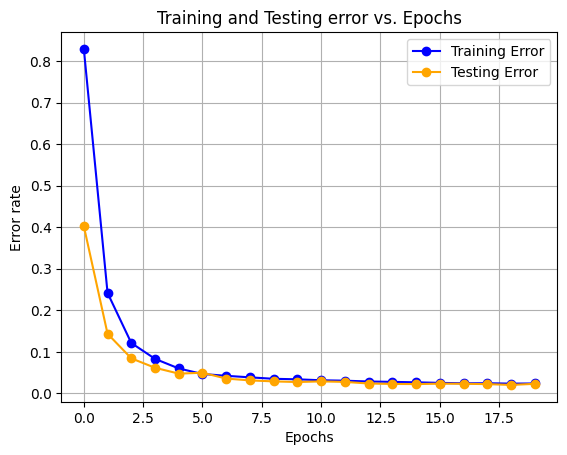
\includegraphics[width=\textwidth]{Assets/graph.png}
        \caption{Training and Testing Error Rates}
        \label{fig:1}
    \end{subfigure}
    \hfill
    \begin{subfigure}{.48\textwidth}
        \centering
        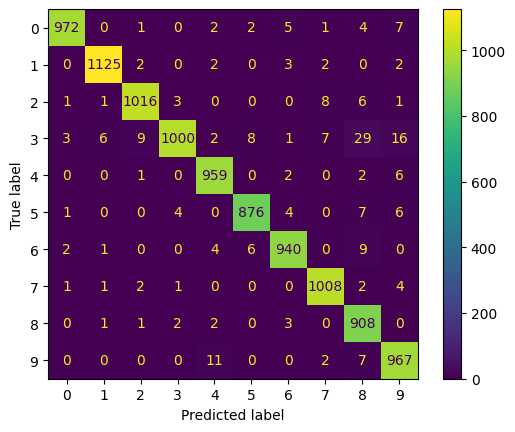
\includegraphics[width=\textwidth]{Assets/confusion-mat.png}
        \caption{Confusion Matrix}
        \label{fig:2}
    \end{subfigure}
    \caption{Training Results}
    \label{fig:results}
\end{figure}

We calculate the most confusing predictions for each class by considering for all examples that were predicted as a particular image and then determining those that were misclassified. From those that were misclassified, we take the image with the the highest confidence. Here, Confidence is calculated
as the distance between the RBF input and center(i.e. the minimum value that determined the predicted class in the first place). So, the most confusing example, or the one with the highest confidence that it is a particular class, but is ultimately wrong, would be the one with the smallest value/RBF distance. The results are shown in
picture \ref{fig:3}. These results make sense. Some prominent example to highlight are a "3" image that was predicted as a 7, and the "8" image that was predicted as a 9. For the "3" image, its understandable that it can be predicted as a 7 because the defining midpoint of the 3 being rather shallow and the top curvature being more than the bottom. For the "8" image, its understandable that it can be predicted as a 9 because the bottom circle looks more filled in, and thus can be seen as a 9.
\begin{figure}[h]
    \centering
    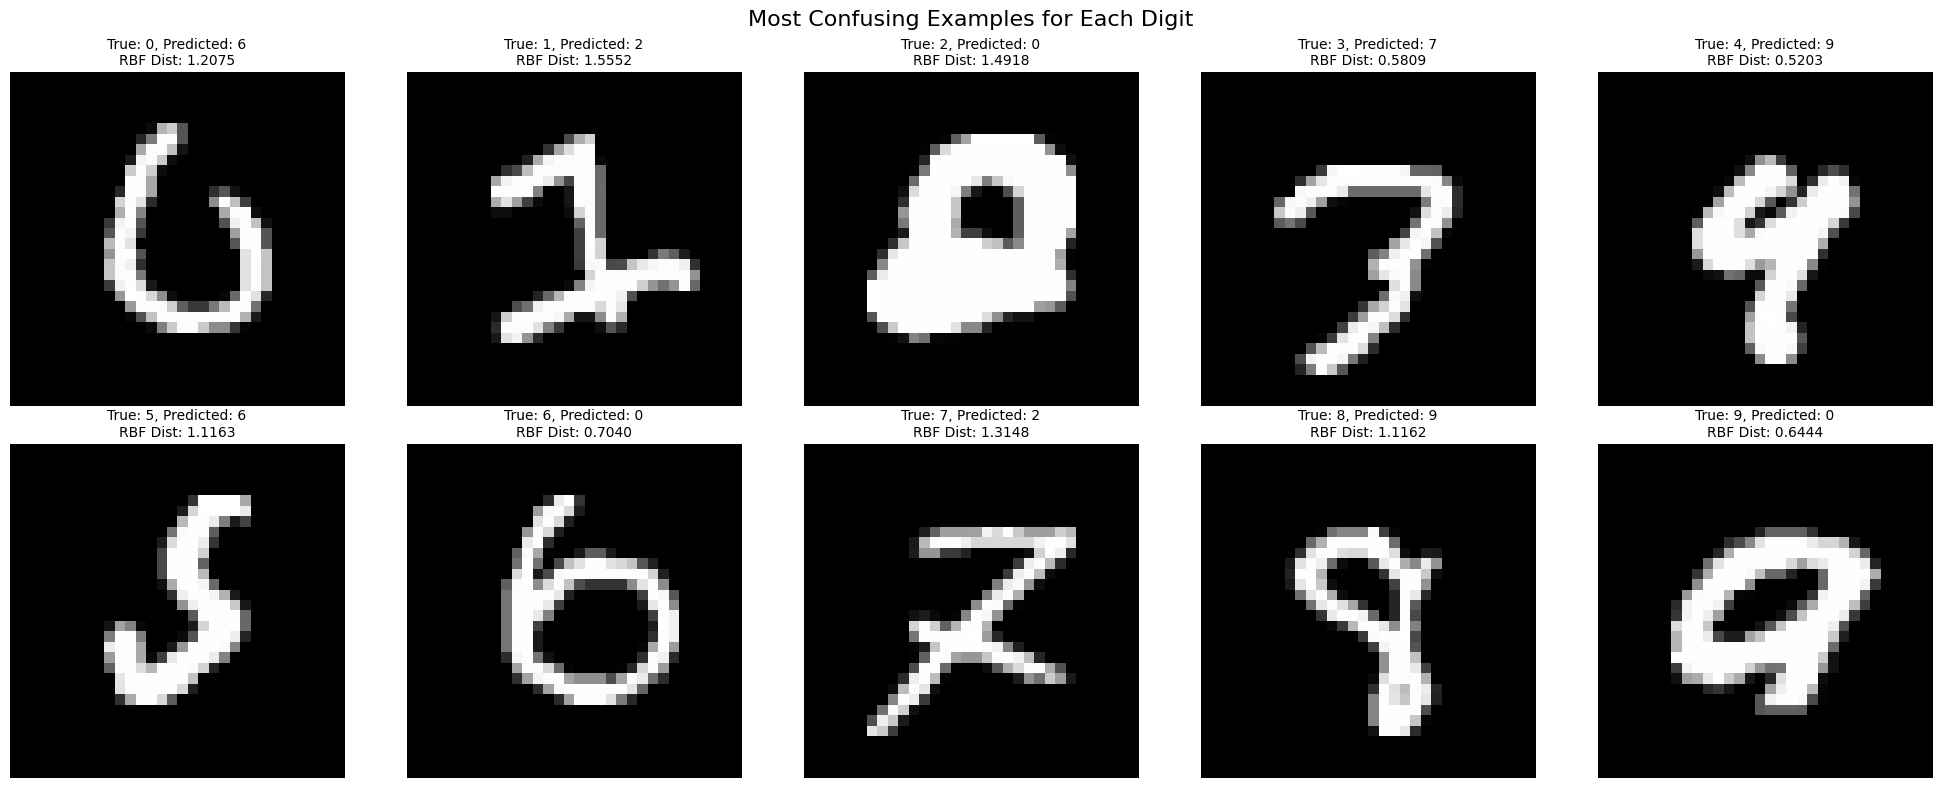
\includegraphics[width=0.7\textwidth]{Assets/most-confusing.png}
    \caption{Most Confusing Predictions}
    \label{fig:3}
\end{figure}

\noindent Our train error rate at epoch 20 was: \textbf{2.22\%}\\
Our test error rate at epoch 20 was: \textbf{2.09\%}

On the ipynb file, you will see these listed as they were training as accuracies. We simply subtracted these accuracies by 1 to get the error rates.

\section{Question 2}

\subsection{2.1}

There were 2 things done to make the model better at transformations:
\begin{itemize}
    \item Data augmentation
    \item Model Architecture changes
\end{itemize}

For data augmentations, we added 60000 more samples to the training dataset using the Affine MNIST dataset.
This dataset consists of 60000 images of the MNIST dataset that have been transformed using
various transformations. The actual zip files consists of 32 different mat files, each with 60000 images, but for simplicity, we chose a singular mat file at random. We used this dataset to augment our training data. This will give the 
model more exposure to how the digits look in different orientations and scales and make it 
generalize better to unseen data. We had also attempted to do some of these transformations ourselves using Transforms.Compose and tried various things such as RandomVerticalFlip, RandomHorizontalFlip, and RandomRotation on the original mnist data. However, this reduced our accuracy to hover around the low 80s at epoch 20. So we decided to append instead the affnist dataset as this would be a way to add more variability, and this seemed to work far better. We also appended 10000 images using the test data of Affnist for our own measurements to test how well the model does overall.

For model architecture changes, we added Batch Normalization layers and dropout layers to the model.

For Batch Normalization, we added these layers after every convolutional layer, but before its passed through to the activation function. The reason this is done is to keep the mean and standard deviation of the outputs close to 0 and 1 respectively. The batch normalization layer is more intricate than just this, but overall, its designed to stabilize the training and make the model more generalizable. Based on our implementation, this seemed to work marginally well by giving percentage increases of 1 to 2 in our accuracies on multiple tests. Obviously for time reasons relating to the training of the model and number of examples, we could not do more thorough tests, but we believe that our model will only benefit from this. We also replaced tanh with a ReLU activation function which showed an increase in model performance as well. The reason we decided to include this was because ReLU is the most popular activation function that is used in industry as well as in literature. The reason this is the case is because of its ability to reduce vanishing gradients as well as being simple and fast. We thought that it would be interesting to try out, because it didn't really get the attention it deserved in the time that Yann LeCun(and others) published this paper. We believe that although Yann LeCun's rationale for using the Tanh function was wuite great, we thought that implementing ReLU instead would be a great complement to the other more modern choices we end up taking explained later.

For Dropout layer, this required a bit more trial and error. We decided to include this a form of regularization. We placed it after the fully connected layer, but before the RBF layer. We initially tested this with a probability of 0.5. This turned out to be too high as it decreased the final accuracy by about 10 percent. There may be a factor to it being that it is pretty close to the end of the neural network, but due to time constraints, we weren't able to test various possibilities regarding the location and number of dropout layers. For the single dropout layer we had, we reduced it to a dropout probability of 0.2, and this provided us with great results

We also experimented with training the Average Pooling Layers to Max Pooling Layers. We decided to keep the trainable weights and biases for max pooling, since we didn't see any detriment from pooling being trainable in general. The reason we decided to swap average pooling out for max pooling is because we think that max pooling will be better at highlighting the stark differences in pixel brightness, that come along with the mnist dataset(black and white).This seemed to work great.

Through this we were able to achieve a .2\% increase in accuracy on the transformed test set, going from
a 97.91\% accuracy using model 1 to a 98.17\% accuracy on model 2. Although this seems slight, we think that given the rather complementary co-development of Lenet5 and MNIST as shown in the original paper, the fact that we introduce more modern blocks and also add affnist to the training data that adds transformations to the mnist dataset(given by professor in assignment), we think this is a satisfactory improvement.

\begin{figure}[h]
    \centering
    \includegraphics[width=0.7\textwidth]{Assets/train2.png}
    \caption{Problem 2 Training and Testing Error Rate}
    \label{fig:3}
\end{figure}
\end{document}